\begin{surferPage}[Chmutov'un Sekizgili]{Bir Chmutov Sekizgili}
Chmutovun sekizgilinde ilk göze çarpan şey ne kadar simetrik olduğu. 
%$\text{Chm}_{d}, \ d=8,$
Bu, denklemine dikkatle bakarak da görülebilir:
    \[T_d(x) + T_d(y) + T_d(z) + 1 = 0;\]
burada $T_d$, Çebişev polinomu olarak adlandırılan ifade (soldaki resim).
$T_8(x)+T_8(y)=0$ ile verilen eğri de sağda resmedilmiş:
    
     \begin{center}
      \begin{tabular}{c@{\quad}c}
        \begin{tabular}{c}
          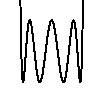
\includegraphics[height=1.75cm]{./../../common/images/Tcheb_008.pdf}
        \end{tabular}    
        &
        \begin{tabular}{c}
          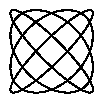
\includegraphics[height=1.75cm]{./../../common/images/Tcheb_2d_008.pdf}
        \end{tabular}    
      \end{tabular}
    \end{center}
    \vspace{-0.3cm}
Bu resimlerden yüzeyin görüntülenen resmine giden yol o kadar da uzun değil.

Bu denklemler 80'lerin başında S.V.\ Chmutov tarafından verilmiştir.
O zamanlarda neredeyse tüm $d$'ler için $\mu(d)$ değerinin dünya rekorlarını,
yani  $d$ dereceli bir yüzeyde olabilecek en fazla tekillik sayısını  veriyorlardı.
90'larda Chmutov kendi dünya rekorunu geliştirdi. 2005 yılındaysa S.~Breske,
    O.~Labs ve D.~van~Straten bu inşayı gerçel yüzeyler üzerinde gerçel tekillikler üretmek için uyarladılar.
\end{surferPage}
